The Canada-France-Hawaii Telescope Lensing Survey (CFHTLenS) represented a major step forward for the field of weak gravitational lensing, in terms of improved accuracy in data reduction \citep{erben/etal:2013}, the implementation of gaussianised matched multi-band photometry \citep{hildebrandt/etal:2012}, cross-correlation clustering analysis between photometric redshift slices to verify tomographic redshift distributions \citep{benjamin/etal:2013}, accurate calibrated shape measurements \citep{miller/etal:2013} and a full suite of informative systematic tests to select a clean data set \citep{heymans/etal:2012}.    Since the public release of this survey in 2013, the community has continued to scrutinise and advance our understanding of CFHTLenS by identifying a number of areas where the analysis could improve:
\begin{itemize}
\item{\citet{choi/etal:2016} identified biases in the tomographic photometric redshift distributions using a more effective clustering analysis, in comparison to \citet{benjamin/etal:2013}, by incorporating newly overlapping spectroscopy from the Sloan Digital Sky Survey.  The CFHTLenS tomographic cosmological analysis was then revisited by \citet{joudaki/etal:2016} in order to include a full redshift error analysis based on the results from \citet{choi/etal:2016}, discussed further in section~\ref{sec:photoz}.}
\item{\citet{asgari/etal:2016} used the stringent `COSEBI' statistic to identify significant non-lensing `B-mode' distortions when the CFHTLenS data was split into tomographic slices.}
\item{\citet{kuijken/etal:2015} showed that the CFHTLenS shear calibration corrections derived in \citet{miller/etal:2013} were underestimated as a result of an imperfect match between the galaxy populations in the data and image simulations.}
\item{\citet{fenechconti/etal:2016} demonstrated that the CFHTLenS data would have been subject to a weight bias that favours galaxies that are more intrinsically oriented with the point-spread function.}
\item{\citet{joudaki/etal:2016} updated the CFHTLenS covariance matrices using larger-box numerical simulations that were less subject to the lack power on large scales.}
\end{itemize}
All these advances in our understanding were incorporated and accounted for in the recent KiDS cosmic shear analysis \citep{hildebrandt/etal:2016} which reports at $2.3 \sigma$ tension with Planck.  Efforts are now underway to fully re-analyse CFHTLenS using the advanced KiDS analysis pipeline with revised shape measurements and calibrations for the shear and photometric redshifts.  

Given the known shortcomings with the original CFHTLenS results, which will impact in different ways on the cosmological conclusions that one can draw from the survey, it is surprising that \citet{kitching/etal:2016} chose to focus their study on the cosmic shear analysis of \citet{kilbinger/etal:2013}.  This is even more unexpected as, out of all the CFHTLenS cosmic shear results, the non-tomographic analysis of \citet{kilbinger/etal:2013} is the least in tension with Planck \citep[see for example][who show that with $\sigma_8 (\Omega_m/0.3)^{0.5} = 0.738^{+0.055}_{-0.032}$, \citet{kilbinger/etal:2013} is in agreement with Planck at $1.6 \sigma$]{abbott/etal:2016}.

\citet{kitching/etal:2016} choose to only vary $\sigma_8$ in their analysis, fixing all other parameters to Planck constraints.  They find a conditional value of $\sigma_8 = 0.789 \pm 0.015$ for their `standard' analysis (row 1 in Table~\ref{tab:Tl_nu}) of the data from \citet{kilbinger/etal:2013}.    We argue that this artificial reduction in the error by a factor of $\sim 3$ could easily mislead, making it appear that the impact of removing all approximations from the theoretical analysis is more significant for current surveys than it is in reality.

We repeated the `one-parameter' analysis for the full range of Limber cases listed in Table~\ref{tab:Tl_nu} finding the lowest conditional value of $\sigma_8 = XXX \pm XXX$ for the XXX case and the highest conditional value of $\sigma_8 = XXX \pm XXX$ for the XXX case.  As expected from the comparison in Figure~\ref{fig:Cl_xi} the different combinations of assuming flat or spherical sky, or baseline of extended Limber make little difference to the cosmological parameter constraints, even in this exaggerated `one-parameter' analysis.  

Our Limber-case findings are therefore in disagreement with \citet{kitching/etal:2016} who find a shift of $\Delta \sigma_8 = 0.007$ between their `standard' analysis (row 1 in Table~\ref{tab:Tl_nu}) and their `Limber' analysis (which we believe corresponds to the Extended Limber spherical case in Table~\ref{tab:Tl_nu}).


\subsection{Comparison of two-point shear statistics; the two-point correlation function, mass aperture statistic and COSEBIS}
\citet{kilbinger/etal:2013} present a detailed comparison of cosmological constraints obtained from a range different two-point shear statistics including the shear correlation function, $\xi_\pm$, the mass aperture statistic, $M_ {\rm ap}^2$ \citep{schneider/etal:1998}, and the COSEBIs statistics \citep{schneider/etal:2010}.  As shown by each statistic's weight function in figure~\ref{fig:filters}, these two-point cosmic shear statistics exhibit different dependences between the angular scales sampled and the $\ell$-range probed.   If a significant bias had been introduced at low-$\ell$ by using flat-sky and Limber approximations, we would then expect to see a systematic shift between the different two-point statistics with the COSEBI statistic being essentially unaffected as it only includes modes with $\ell \gtrsim 80$.  This is found not to be the case with all three statistics finding $\sigma_8 (\Omega_m/0.27)^\alpha = 0.79$ with errors that range from $0.03$ to $0.06$ \citep[see Table 5 of][]{kilbinger/etal:2013}.  This comparison further supports our argument that the approximations highlighted by \citet{kitching/etal:2016} have negligible impact for current surveys.

\begin{figure}[htb]
\begin{center}
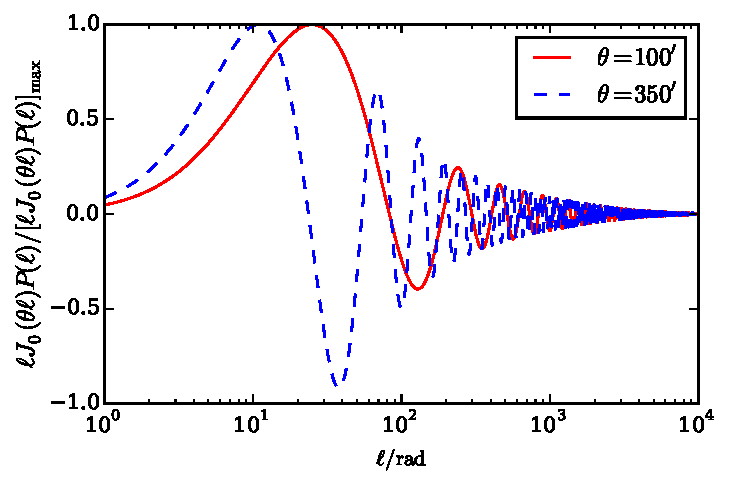
\includegraphics[width=0.5\textwidth]{figures/IntegKsip.pdf}\\
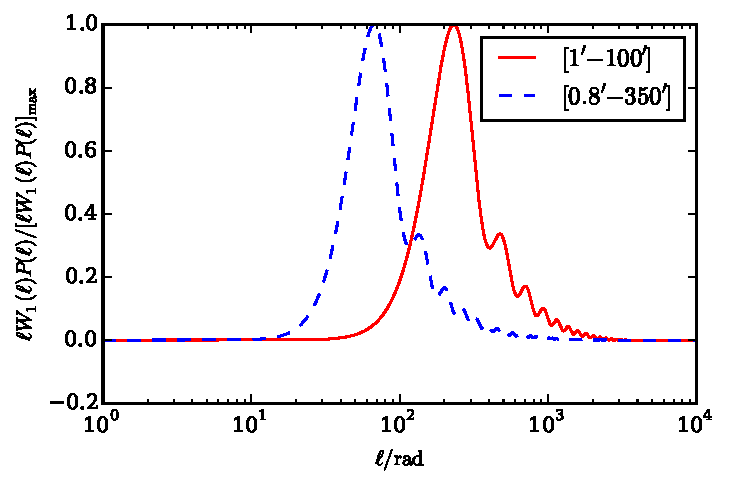
\includegraphics[width=0.5\textwidth]{figures/IntegCOSEBIs.pdf}\\
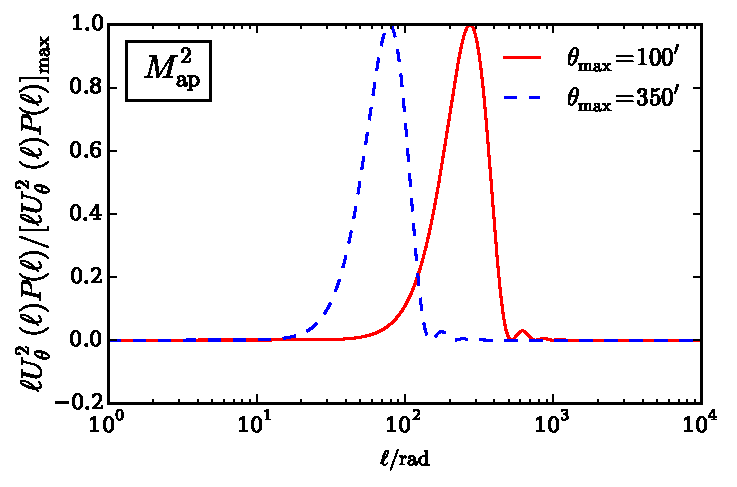
\includegraphics[width=0.5\textwidth]{figures/IntegMap.pdf}
\caption{ \label{fig:filters}. Integrand of $\xi_+$, $E_1$ and $M_{\rm ap}$.
All the values are normalized with respect to their maximum value. Two cases are shown for each statistic. 
For COSEBIs this is an angular range indicated in the caption. For aperture mass statistic $\theta_{\rm max}=2\theta$ is shown.
}
\end{center}
\end{figure}





